%
% dutchroll.tex -- Dutch Roll, Front- und Draufsicht
%
% (c) 2026 OST Ostschweizer Fachhochschule
%
\documentclass[tikz]{standalone}
\usepackage{amsmath}
\usepackage{times}
\usepackage{txfonts}
\usepackage{graphicx}
\usetikzlibrary{arrows,calc}
\definecolor{darkred}{rgb}{0.8,0,0}
\definecolor{darkgreen}{rgb}{0,0.6,0}
\begin{document}
\begin{tikzpicture}[>=latex]
\node[anchor=south west,inner sep=0] (bild) at (0,0)
	{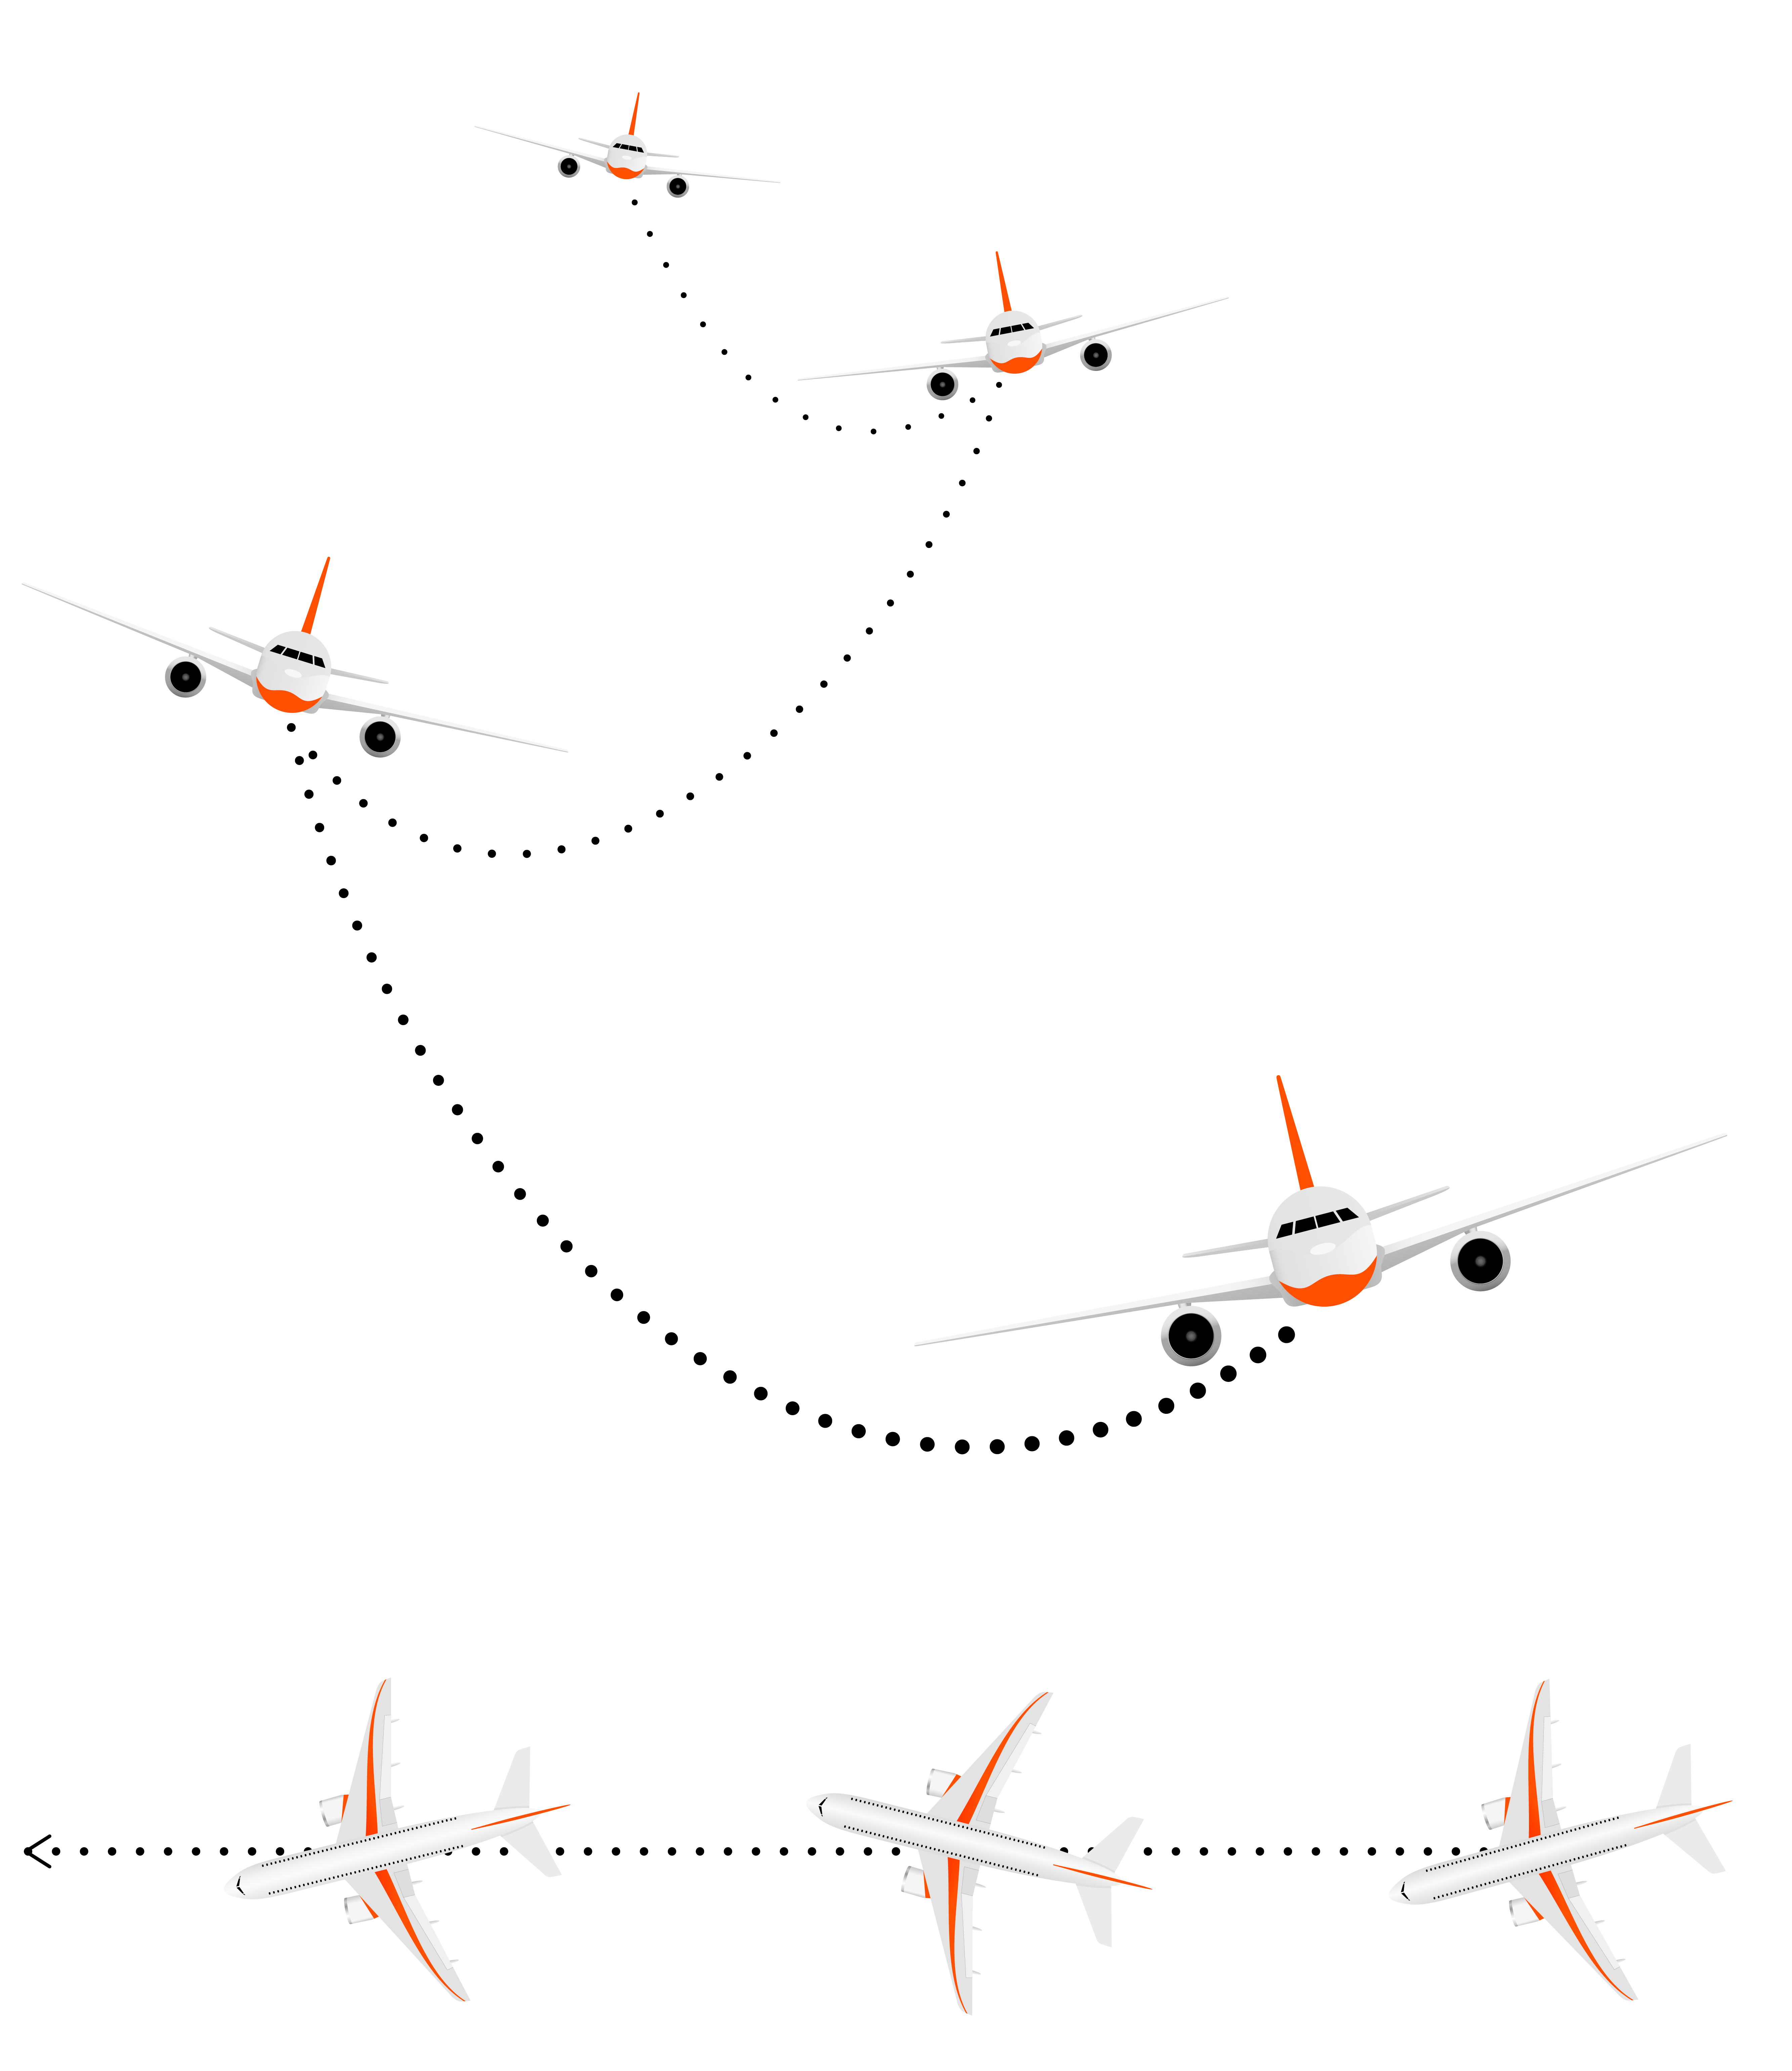
\includegraphics[width=10cm]{dutchroll-transparent.png}};
\begin{scope}[x={(bild.south east)},y={(bild.north west)}]
	\node[anchor=south] at (0.50,0.98) {Frontansicht (Front View)};
	\node at (0.50,0.217) {Draufsicht (Top View)};
\end{scope}
\end{tikzpicture}
\end{document}
